\PassOptionsToPackage{table}{xcolor}
\documentclass[12pt,letterpaper,twocolumn,openany,nodeprecatedcode,bg=none]{dndbook}
\usepackage[english]{babel}
\usepackage[utf8]{inputenc}
\usepackage{longtable,booktabs,array}
\usepackage{calc}
\usepackage{etoolbox}
\usepackage{caption}
\usepackage{float}
\usepackage{graphicx}
\usepackage{needspace}
\usepackage{tikz}

% Reset zebra striping at the start of every table
\AtBeginEnvironment{longtable}{\rowcolors{1}{white}{gray!10}\small}
\AtBeginEnvironment{table}{\rowcolors{1}{white}{gray!10}}

\providecommand{\pandocbounded}[1]{#1}
\providecommand{\tightlist}{%
  \setlength{\itemsep}{0pt}\setlength{\parskip}{0pt}}

\captionsetup{labelformat=empty}
\setcounter{secnumdepth}{0}
\setlength{\parindent}{0pt}
\setlength{\parskip}{0.5\baselineskip}
\setlength{\headheight}{15pt}

% Prevent orphaned subsections
\let\oldsubsection\subsection
\renewcommand{\subsection}[1]{%
  \needspace{5\baselineskip}%
  \oldsubsection{#1}%
}

\begin{document}
\onecolumn

      \title{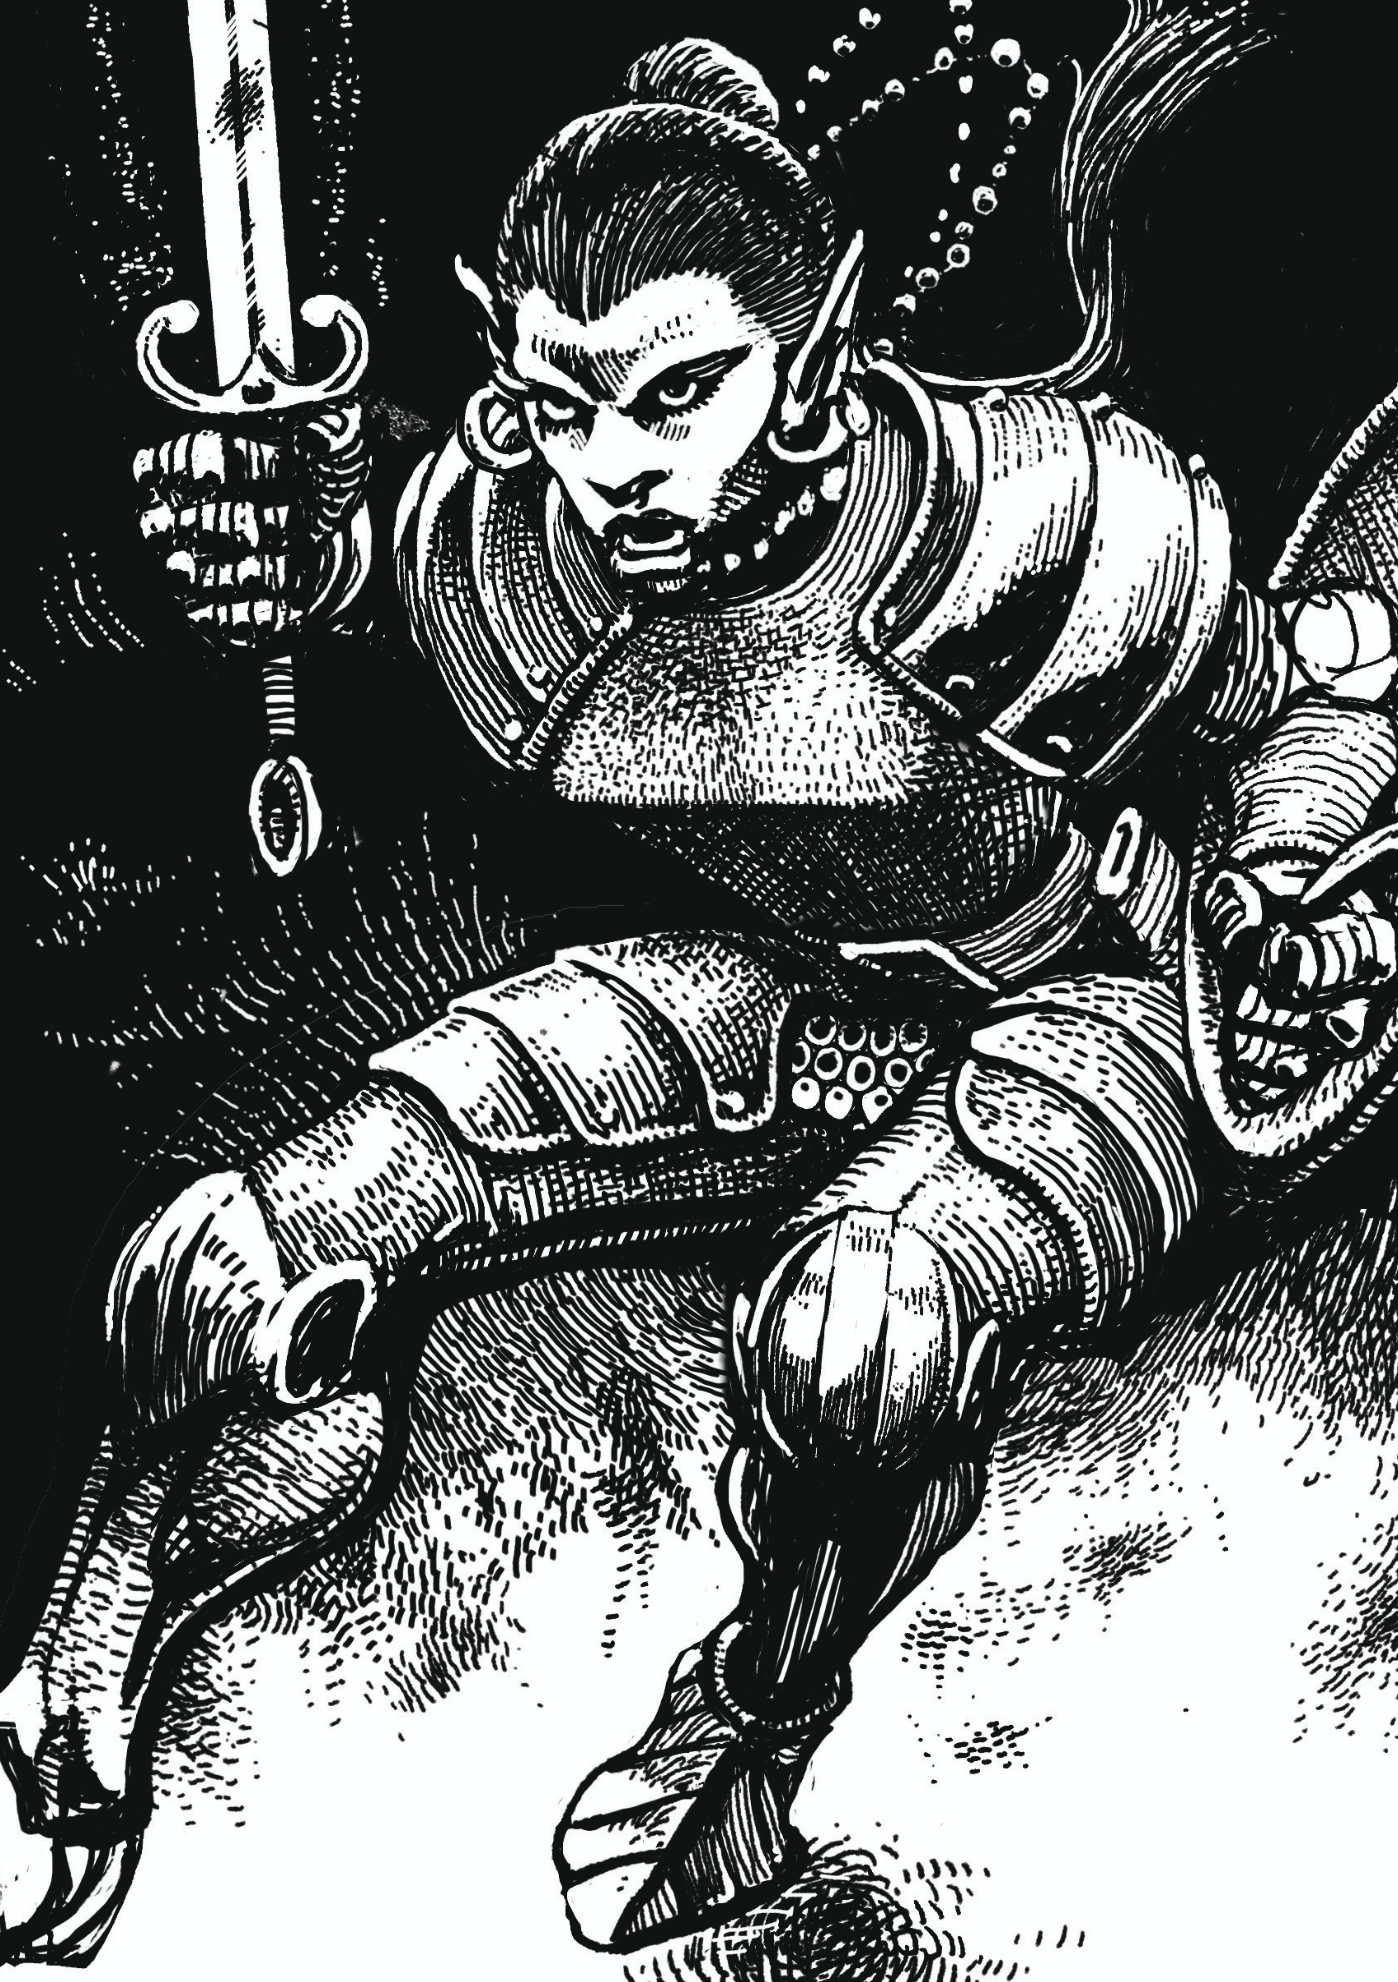
\includegraphics[width=0.9\textwidth,height=0.55\textheight,keepaspectratio]{orcFighter.png}\\[1.5cm]Fighter}
  \author{Class Handbook}
\date{}
\maketitle



\clearpage
\twocolumn

\section{Fighter}\label{fighter}

\subsection{Core Fighter Traits}\label{core-fighter-traits}

\needspace{11\baselineskip}

{\def\LTcaptype{none} % do not increment counter
\begin{table}[!htbp]
\centering
\begin{tabular}{@{}
  >{\raggedright\arraybackslash}p{(\linewidth - 2\tabcolsep) * \real{0.3250}}
  >{\raggedright\arraybackslash}p{(\linewidth - 2\tabcolsep) * \real{0.6750}}@{}}
\toprule\noalign{}
\begin{minipage}[b]{\linewidth}\raggedright
\textbf{Primary Ability}
\end{minipage} & \begin{minipage}[b]{\linewidth}\raggedright
Strength
\end{minipage} \\
\midrule\noalign{}
\textbf{Hit Points} & 1d8 \\
\textbf{Saving Throw Proficiencies} & Strength, Dexterity,
Constitution \\
\textbf{Skill Proficiencies} & Choose 2 skills \\
\textbf{Weapon Proficiencies} & Choose 4 categories \\
\textbf{Starting Equipment} & Chain Mail, Open Helm, Greatsword, Sabre,
Large Shield \\
\bottomrule\noalign{}
\end{tabular}
\end{table}
}

\subsection{Fighter Features}\label{fighter-features}

\needspace{20\baselineskip}

{\def\LTcaptype{none} % do not increment counter
\begin{table}[!htbp]
\centering
\begin{tabular}{@{}
  >{\raggedright\arraybackslash}p{(\linewidth - 4\tabcolsep) * \real{0.0943}}
  >{\raggedright\arraybackslash}p{(\linewidth - 4\tabcolsep) * \real{0.2075}}
  >{\raggedright\arraybackslash}p{(\linewidth - 4\tabcolsep) * \real{0.6981}}@{}}
\toprule\noalign{}
\begin{minipage}[b]{\linewidth}\raggedright
Level
\end{minipage} & \begin{minipage}[b]{\linewidth}\raggedright
Proficiency
\end{minipage} & \begin{minipage}[b]{\linewidth}\raggedright
Class Features
\end{minipage} \\
\midrule\noalign{}
1 & +2 & Weapon Specialization, Fighting Style \\
2 & +2 & --- \\
3 & +2 & Specialist Attack, Ability Bonus \\
4 & +2 & --- \\
5 & +2 & Two Attacks \\
6 & +2 & --- \\
7 & +2 & Ability Bonus \\
8 & +2 & --- \\
9 & +3 & Three Attacks \\
10 & +3 & --- \\
\bottomrule\noalign{}
\end{tabular}
\end{table}
}

\subsection{Level 1: Weapon
Specialization}\label{level-1-weapon-specialization}

Pick a weapon you are proficient with. You add your proficiency bonus to
damage rolls with it. After an extended period of downtime, you can swap
this choice to a different weapon.

\subsection{Level 1: Fighting Style}\label{level-1-fighting-style}

You are trained in one specific style of fighting.

\begin{itemize}
\tightlist
\item
  \textbf{Bulwark.} Once per turn when a hostile creature in melee range
  attempts to move, it must make a Dexterity saving throw (DC 8 + your
  proficiency bonus + your Strength modifier). If it fails, it cannot
  move that turn.
\item
  \textbf{Berserker.} Once per turn when you drop a target to 0 hit
  points with an attack, you may make one additional attack.
\item
  \textbf{Duelist.} While wielding a weapon you are proficient with, you
  can impose disadvantage on one melee attack made against you per
  round.
\item
  \textbf{Guardian.} You gain +1 AC. If a hostile creature in melee
  range attacks, you may choose its target. You must choose a creature
  hostile to it, such as yourself.
\item
  \textbf{Monster Slayer.} You gain a +2 bonus to damage rolls against
  creatures that are larger than you.
\item
  \textbf{Sharpshooter.} You add your proficiency bonus twice to attack
  rolls with ranged attacks.
\item
  \textbf{Stalwart.} You gain a bonus to your maximum hit points equal
  to your level. While you are at half hit points or less, you regain
  hit points at the start of your turn equal to your Constitution
  modifier.
\item
  \textbf{Warrior Mage.} You gain a wizard cantrip of your choice and
  can cast one 1st level wizard spell once per long rest. Each time you
  gain a level, you can swap those choices for different options. You
  use the rules for casting spells as per the wizard class.
\end{itemize}

\subsection{Level 3: Specialist Attack}\label{level-3-specialist-attack}

The first time you miss an attack on your turn, reroll the attack. If
you have disadvantage or advantage, reroll one or both dice.

\subsection{Level 3: Ability Bonus}\label{level-3-ability-bonus}

You gain a +1 bonus to two different abilities of your choice.

\subsection{Level 5: Two Attacks}\label{level-5-two-attacks}

When you attack, you can make two weapon attacks.

\subsection{Level 7: Ability Bonus}\label{level-7-ability-bonus}

You gain a +1 bonus to two different abilities of your choice.

\subsection{Level 9: Three Attacks}\label{level-9-three-attacks}

When you attack, you can make three weapon attacks.

\onecolumn

\clearpage
\thispagestyle{empty}
\begin{center}
\vspace*{\fill}
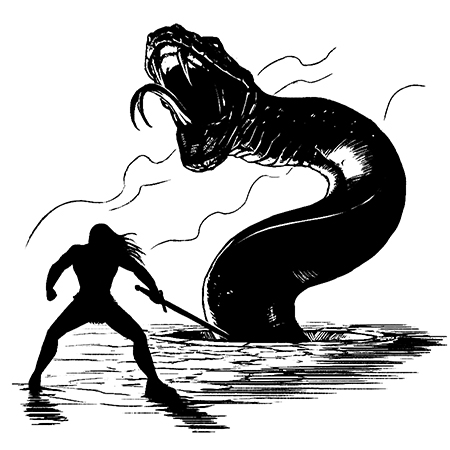
\includegraphics[width=0.7\textwidth,keepaspectratio]{monsterHunter.jpg}\par
\vspace{0.4cm}
{\itshape A fighter stands tall against all odds.}\par
\vspace*{\fill}
\end{center}

\end{document}